%%%%%%%%%%%%%%%%%%%%%%%%%%%%%%%%%%%%%%%%%
% University Assignment Title Page 
% LaTeX Template
% Version 1.0 (27/12/12)
%
% This template has been downloaded from:
% http://www.LaTeXTemplates.com
%
% Original author:
% WikiBooks (http://en.wikibooks.org/wiki/LaTeX/Title_Creation)
%
% License:
% CC BY-NC-SA 3.0 (http://creativecommons.org/licenses/by-nc-sa/3.0/)
% 
% Instructions for using this template:
% This title page is capable of being compiled as is. This is not useful for 
% including it in another document. To do this, you have two options: 
%
% 1) Copy/paste everything between \begin{document} and \end{document} 
% starting at \begin{titlepage} and paste this into another LaTeX file where you 
% want your title page.
% OR
% 2) Remove everything outside the \begin{titlepage} and \end{titlepage} and 
% move this file to the same directory as the LaTeX file you wish to add it to. 
% Then add %%%%%%%%%%%%%%%%%%%%%%%%%%%%%%%%%%%%%%%%%
% University Assignment Title Page 
% LaTeX Template
% Version 1.0 (27/12/12)
%
% This template has been downloaded from:
% http://www.LaTeXTemplates.com
%
% Original author:
% WikiBooks (http://en.wikibooks.org/wiki/LaTeX/Title_Creation)
%
% License:
% CC BY-NC-SA 3.0 (http://creativecommons.org/licenses/by-nc-sa/3.0/)
% 
% Instructions for using this template:
% This title page is capable of being compiled as is. This is not useful for 
% including it in another document. To do this, you have two options: 
%
% 1) Copy/paste everything between \begin{document} and \end{document} 
% starting at \begin{titlepage} and paste this into another LaTeX file where you 
% want your title page.
% OR
% 2) Remove everything outside the \begin{titlepage} and \end{titlepage} and 
% move this file to the same directory as the LaTeX file you wish to add it to. 
% Then add %%%%%%%%%%%%%%%%%%%%%%%%%%%%%%%%%%%%%%%%%
% University Assignment Title Page 
% LaTeX Template
% Version 1.0 (27/12/12)
%
% This template has been downloaded from:
% http://www.LaTeXTemplates.com
%
% Original author:
% WikiBooks (http://en.wikibooks.org/wiki/LaTeX/Title_Creation)
%
% License:
% CC BY-NC-SA 3.0 (http://creativecommons.org/licenses/by-nc-sa/3.0/)
% 
% Instructions for using this template:
% This title page is capable of being compiled as is. This is not useful for 
% including it in another document. To do this, you have two options: 
%
% 1) Copy/paste everything between \begin{document} and \end{document} 
% starting at \begin{titlepage} and paste this into another LaTeX file where you 
% want your title page.
% OR
% 2) Remove everything outside the \begin{titlepage} and \end{titlepage} and 
% move this file to the same directory as the LaTeX file you wish to add it to. 
% Then add %%%%%%%%%%%%%%%%%%%%%%%%%%%%%%%%%%%%%%%%%
% University Assignment Title Page 
% LaTeX Template
% Version 1.0 (27/12/12)
%
% This template has been downloaded from:
% http://www.LaTeXTemplates.com
%
% Original author:
% WikiBooks (http://en.wikibooks.org/wiki/LaTeX/Title_Creation)
%
% License:
% CC BY-NC-SA 3.0 (http://creativecommons.org/licenses/by-nc-sa/3.0/)
% 
% Instructions for using this template:
% This title page is capable of being compiled as is. This is not useful for 
% including it in another document. To do this, you have two options: 
%
% 1) Copy/paste everything between \begin{document} and \end{document} 
% starting at \begin{titlepage} and paste this into another LaTeX file where you 
% want your title page.
% OR
% 2) Remove everything outside the \begin{titlepage} and \end{titlepage} and 
% move this file to the same directory as the LaTeX file you wish to add it to. 
% Then add \input{./title_page_1.tex} to your LaTeX file where you want your
% title page.
%
% In this example, we are using the 2nd method. You cannot compile this docuent by itself, since there is no '\begin|end{document}. You must compile the main document which calls this document.
%
%%%%%%%%%%%%%%%%%%%%%%%%%%%%%%%%%%%%%%%%%

%----------------------------------------------------------------------------------------
%	PACKAGES AND OTHER DOCUMENT CONFIGURATIONS
%----------------------------------------------------------------------------------------

%\documentclass[12pt]{article}
%
%\begin{document}

\begin{titlepage}

\newcommand{\HRule}{\rule{\linewidth}{0.5mm}} % Defines a new command for the horizontal lines, change thickness here

\center % Center everything on the page
 
%----------------------------------------------------------------------------------------
%	HEADING SECTIONS
%----------------------------------------------------------------------------------------
%
% The \\[metric] refers to the spacing after the text.
\textsc{\LARGE Linux System Administration}\\[1.5cm] % Name of your university/college
\textsc{\Large RHEL, CentOS, Fedora}\\[1.0cm] % Major heading such as course name
\textsc{\large Command Line Reference}\\[0.5cm] % Minor heading such as course title

%----------------------------------------------------------------------------------------
%	TITLE SECTION
%----------------------------------------------------------------------------------------

\HRule \\[0.4cm]
{ \huge \bfseries Linux System Administration}\footnote{This book is not intended for 19\textsuperscript{th} century textile workers or climate change deniers.}\\[0.4cm] % Title of your document
\HRule \\[1.5cm]
 
%----------------------------------------------------------------------------------------
%	AUTHOR SECTION
%----------------------------------------------------------------------------------------
%
% minipage is used when you want to place side by side two items, as in this case, or as in placing two pictures or tables side by side
%
\begin{minipage}{0.4\textwidth} % means .4 or 40% of textwidth, the width of the minipage
\begin{flushleft} \large
\emph{Author:}\\ % emph = emphasis or italics
Murray \textsc{davis} % Your name and \textsc = text_small_caps
\end{flushleft}
\end{minipage}
~
\begin{minipage}{0.4\textwidth}
\begin{flushright} \large
\emph{Topic:} \\
Linux \textsc{System Administration Version \versionnumber} 
\end{flushright}
\end{minipage}\\[4cm]

% If you don't want a supervisor, uncomment the two lines below and remove the section above
%\Large \emph{Author:}\\
%John \textsc{Smith}\\[3cm] % Your name

%----------------------------------------------------------------------------------------
%	DATE SECTION
%----------------------------------------------------------------------------------------

{\large \today{ - Compile Date } \textsl{November 3, 2016 - Revision Date}}\\[3cm] % Date, change the \today to a set date if you want to be precise

%----------------------------------------------------------------------------------------
%	LOGO SECTION
%----------------------------------------------------------------------------------------
%
% Note: The file is in the folder called figures that lies in the main directory. The file is called: cube.png, but you do not have to supply the filename extension '.png'.
%
\begin{figure}[!h]
\centering
\href{https://en.wikipedia.org/wiki/Luddite}{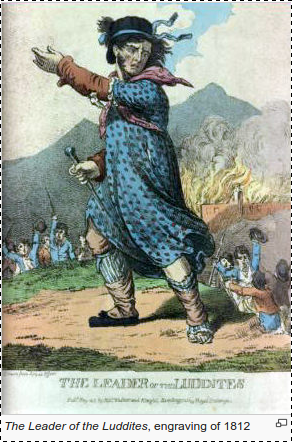
\includegraphics[width=0.2\textwidth]{figures/ludite_leader}}
\caption{The leader of the Ludites}
\label{title_page_1_ludites}
\end{figure}
 
%----------------------------------------------------------------------------------------

\vfill % Fill the rest of the page with whitespace

\end{titlepage} to your LaTeX file where you want your
% title page.
%
% In this example, we are using the 2nd method. You cannot compile this docuent by itself, since there is no '\begin|end{document}. You must compile the main document which calls this document.
%
%%%%%%%%%%%%%%%%%%%%%%%%%%%%%%%%%%%%%%%%%

%----------------------------------------------------------------------------------------
%	PACKAGES AND OTHER DOCUMENT CONFIGURATIONS
%----------------------------------------------------------------------------------------

%\documentclass[12pt]{article}
%
%\begin{document}

\begin{titlepage}

\newcommand{\HRule}{\rule{\linewidth}{0.5mm}} % Defines a new command for the horizontal lines, change thickness here

\center % Center everything on the page
 
%----------------------------------------------------------------------------------------
%	HEADING SECTIONS
%----------------------------------------------------------------------------------------
%
% The \\[metric] refers to the spacing after the text.
\textsc{\LARGE Linux System Administration}\\[1.5cm] % Name of your university/college
\textsc{\Large RHEL, CentOS, Fedora}\\[1.0cm] % Major heading such as course name
\textsc{\large Command Line Reference}\\[0.5cm] % Minor heading such as course title

%----------------------------------------------------------------------------------------
%	TITLE SECTION
%----------------------------------------------------------------------------------------

\HRule \\[0.4cm]
{ \huge \bfseries Linux System Administration}\footnote{This book is not intended for 19\textsuperscript{th} century textile workers or climate change deniers.}\\[0.4cm] % Title of your document
\HRule \\[1.5cm]
 
%----------------------------------------------------------------------------------------
%	AUTHOR SECTION
%----------------------------------------------------------------------------------------
%
% minipage is used when you want to place side by side two items, as in this case, or as in placing two pictures or tables side by side
%
\begin{minipage}{0.4\textwidth} % means .4 or 40% of textwidth, the width of the minipage
\begin{flushleft} \large
\emph{Author:}\\ % emph = emphasis or italics
Murray \textsc{davis} % Your name and \textsc = text_small_caps
\end{flushleft}
\end{minipage}
~
\begin{minipage}{0.4\textwidth}
\begin{flushright} \large
\emph{Topic:} \\
Linux \textsc{System Administration Version \versionnumber} 
\end{flushright}
\end{minipage}\\[4cm]

% If you don't want a supervisor, uncomment the two lines below and remove the section above
%\Large \emph{Author:}\\
%John \textsc{Smith}\\[3cm] % Your name

%----------------------------------------------------------------------------------------
%	DATE SECTION
%----------------------------------------------------------------------------------------

{\large \today{ - Compile Date } \textsl{November 3, 2016 - Revision Date}}\\[3cm] % Date, change the \today to a set date if you want to be precise

%----------------------------------------------------------------------------------------
%	LOGO SECTION
%----------------------------------------------------------------------------------------
%
% Note: The file is in the folder called figures that lies in the main directory. The file is called: cube.png, but you do not have to supply the filename extension '.png'.
%
\begin{figure}[!h]
\centering
\href{https://en.wikipedia.org/wiki/Luddite}{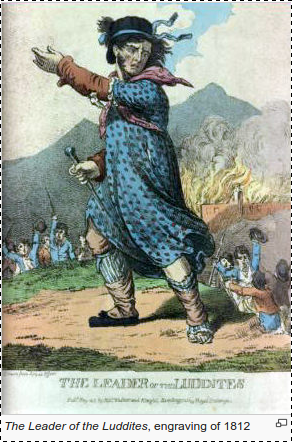
\includegraphics[width=0.2\textwidth]{figures/ludite_leader}}
\caption{The leader of the Ludites}
\label{title_page_1_ludites}
\end{figure}
 
%----------------------------------------------------------------------------------------

\vfill % Fill the rest of the page with whitespace

\end{titlepage} to your LaTeX file where you want your
% title page.
%
% In this example, we are using the 2nd method. You cannot compile this docuent by itself, since there is no '\begin|end{document}. You must compile the main document which calls this document.
%
%%%%%%%%%%%%%%%%%%%%%%%%%%%%%%%%%%%%%%%%%

%----------------------------------------------------------------------------------------
%	PACKAGES AND OTHER DOCUMENT CONFIGURATIONS
%----------------------------------------------------------------------------------------

%\documentclass[12pt]{article}
%
%\begin{document}

\begin{titlepage}

\newcommand{\HRule}{\rule{\linewidth}{0.5mm}} % Defines a new command for the horizontal lines, change thickness here

\center % Center everything on the page
 
%----------------------------------------------------------------------------------------
%	HEADING SECTIONS
%----------------------------------------------------------------------------------------
%
% The \\[metric] refers to the spacing after the text.
\textsc{\LARGE Linux System Administration}\\[1.5cm] % Name of your university/college
\textsc{\Large RHEL, CentOS, Fedora}\\[1.0cm] % Major heading such as course name
\textsc{\large Command Line Reference}\\[0.5cm] % Minor heading such as course title

%----------------------------------------------------------------------------------------
%	TITLE SECTION
%----------------------------------------------------------------------------------------

\HRule \\[0.4cm]
{ \huge \bfseries Linux System Administration}\footnote{This book is not intended for 19\textsuperscript{th} century textile workers or climate change deniers.}\\[0.4cm] % Title of your document
\HRule \\[1.5cm]
 
%----------------------------------------------------------------------------------------
%	AUTHOR SECTION
%----------------------------------------------------------------------------------------
%
% minipage is used when you want to place side by side two items, as in this case, or as in placing two pictures or tables side by side
%
\begin{minipage}{0.4\textwidth} % means .4 or 40% of textwidth, the width of the minipage
\begin{flushleft} \large
\emph{Author:}\\ % emph = emphasis or italics
Murray \textsc{davis} % Your name and \textsc = text_small_caps
\end{flushleft}
\end{minipage}
~
\begin{minipage}{0.4\textwidth}
\begin{flushright} \large
\emph{Topic:} \\
Linux \textsc{System Administration Version \versionnumber} 
\end{flushright}
\end{minipage}\\[4cm]

% If you don't want a supervisor, uncomment the two lines below and remove the section above
%\Large \emph{Author:}\\
%John \textsc{Smith}\\[3cm] % Your name

%----------------------------------------------------------------------------------------
%	DATE SECTION
%----------------------------------------------------------------------------------------

{\large \today{ - Compile Date } \textsl{November 3, 2016 - Revision Date}}\\[3cm] % Date, change the \today to a set date if you want to be precise

%----------------------------------------------------------------------------------------
%	LOGO SECTION
%----------------------------------------------------------------------------------------
%
% Note: The file is in the folder called figures that lies in the main directory. The file is called: cube.png, but you do not have to supply the filename extension '.png'.
%
\begin{figure}[!h]
\centering
\href{https://en.wikipedia.org/wiki/Luddite}{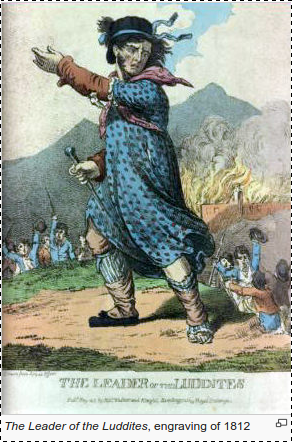
\includegraphics[width=0.2\textwidth]{figures/ludite_leader}}
\caption{The leader of the Ludites}
\label{title_page_1_ludites}
\end{figure}
 
%----------------------------------------------------------------------------------------

\vfill % Fill the rest of the page with whitespace

\end{titlepage} to your LaTeX file where you want your
% title page.
%
% In this example, we are using the 2nd method. You cannot compile this docuent by itself, since there is no '\begin|end{document}. You must compile the main document which calls this document.
%
%%%%%%%%%%%%%%%%%%%%%%%%%%%%%%%%%%%%%%%%%

%----------------------------------------------------------------------------------------
%	PACKAGES AND OTHER DOCUMENT CONFIGURATIONS
%----------------------------------------------------------------------------------------

%\documentclass[12pt]{article}
%
%\begin{document}

\begin{titlepage}

\newcommand{\HRule}{\rule{\linewidth}{0.5mm}} % Defines a new command for the horizontal lines, change thickness here

\center % Center everything on the page
 
%----------------------------------------------------------------------------------------
%	HEADING SECTIONS
%----------------------------------------------------------------------------------------
%
% The \\[metric] refers to the spacing after the text.
\textsc{\LARGE Linux System Administration}\\[1.5cm] % Name of your university/college
\textsc{\Large RHEL, CentOS, Fedora}\\[1.0cm] % Major heading such as course name
\textsc{\large Command Line Reference}\\[0.5cm] % Minor heading such as course title

%----------------------------------------------------------------------------------------
%	TITLE SECTION
%----------------------------------------------------------------------------------------

\HRule \\[0.4cm]
{ \huge \bfseries Linux System Administration}\footnote{This book is not intended for 19\textsuperscript{th} century textile workers or climate change deniers.}\\[0.4cm] % Title of your document
\HRule \\[1.5cm]
 
%----------------------------------------------------------------------------------------
%	AUTHOR SECTION
%----------------------------------------------------------------------------------------
%
% minipage is used when you want to place side by side two items, as in this case, or as in placing two pictures or tables side by side
%
\begin{minipage}{0.4\textwidth} % means .4 or 40% of textwidth, the width of the minipage
\begin{flushleft} \large
\emph{Author:}\\ % emph = emphasis or italics
Murray \textsc{davis} % Your name and \textsc = text_small_caps
\end{flushleft}
\end{minipage}
~
\begin{minipage}{0.4\textwidth}
\begin{flushright} \large
\emph{Topic:} \\
Linux \textsc{System Administration Version \versionnumber} 
\end{flushright}
\end{minipage}\\[4cm]

% If you don't want a supervisor, uncomment the two lines below and remove the section above
%\Large \emph{Author:}\\
%John \textsc{Smith}\\[3cm] % Your name

%----------------------------------------------------------------------------------------
%	DATE SECTION
%----------------------------------------------------------------------------------------

{\large \today{ - Compile Date } \textsl{November 3, 2016 - Revision Date}}\\[3cm] % Date, change the \today to a set date if you want to be precise

%----------------------------------------------------------------------------------------
%	LOGO SECTION
%----------------------------------------------------------------------------------------
%
% Note: The file is in the folder called figures that lies in the main directory. The file is called: cube.png, but you do not have to supply the filename extension '.png'.
%
\begin{figure}[!h]
\centering
\href{https://en.wikipedia.org/wiki/Luddite}{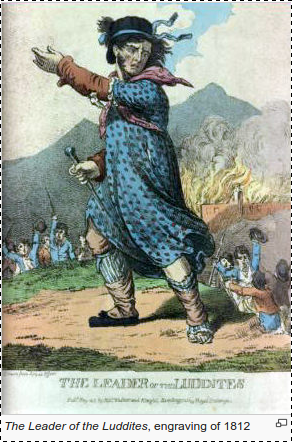
\includegraphics[width=0.2\textwidth]{figures/ludite_leader}}
\caption{The leader of the Ludites}
\label{title_page_1_ludites}
\end{figure}
 
%----------------------------------------------------------------------------------------

\vfill % Fill the rest of the page with whitespace

\end{titlepage}